
\documentclass[12pt]{article}
\usepackage{amsmath}
\DeclareMathOperator*{\argmin}{arg\,min} % thin space, limits underneath in displays
\DeclareMathOperator*{\argmax}{arg\,max} % thin space, limits underneath in displays
\newtheorem{thm}{Theorem}
\usepackage{amssymb}
\usepackage{amsfonts}
\usepackage{mathrsfs}
\usepackage{bm}
\usepackage{indentfirst}
\setlength{\parindent}{0em}
\usepackage[margin=1in]{geometry}
\usepackage{graphicx}
\usepackage{setspace}
\doublespacing
\usepackage[flushleft]{threeparttable}
\usepackage{booktabs,caption}
\usepackage{float}
\usepackage{graphicx}

\usepackage{import}
\usepackage{xifthen}
\usepackage{pdfpages}
\usepackage{transparent}

\newcommand{\incfig}[1]{%
\def\svgwidth{\columnwidth}
\import{./figures/}{#1.pdf_tex}
}


\usepackage{graphicx}
\usepackage{xspace,color}
\usepackage{url}
\usepackage{listings}


\lstset{commentstyle=\color{gray},keywordstyle=\color{black},
showstringspaces=false, basicstyle = \small
} %% basicstyle set fontsize
\lstnewenvironment{rc}[1][]{\lstset{language=R}}{}
\newcommand{\ri}[1]{\lstinline{#1}}  %% Short for 'R inline'



\lstdefinelanguage{language=R}{
numbers=left,
numberstyle=\footnotesize,
numbersep=1em,
xleftmargin=1em,
framextopmargin=2em,
framexbottommargin=2em,
showspaces=false,
showtabs=false,
showstringspaces=false,
frame=l,
tabsize=4,
}



\title{Linear Regression}
\author{Synferlo}
\date{May, 10}


\begin{document}
\maketitle
\newpage



\section{Simple Linear Regression}

\subsection{Estimation}

\begin{equation*}
 \widehat{y} =  \widehat{\beta_0} +  \widehat{\beta_1} x
\end{equation*}

\begin{equation*}
 \widehat{\beta_1} = \rho_{xy} \frac{s_{y}}{s_{x}},
 \text{ and }  \widehat{\beta_0} =  \overline{y} -  \widehat{\beta_1}
   \overline{x}
\end{equation*}

$  \overline{x},  \overline{y} $: sample means\\
$ s_{x}, s_{y} $: sample standard deviation\\
$ \rho_{xy} $: the estimate of correlation between $ X $ and $ Y $
based on the data.\\



\subsection{Statistical Inference}

\begin{table}[h!]
\begin{center}
	
\begin{threeparttable}
		\caption{Price and Volume (unnormalized result)}			

\begin{tabular}{lllll}
\\ [-1.8ex]
\hline
\hline \\[-1.8ex]
 & {\textbf {Coefs}} & {\textbf {SE}} & {\textbf {t-value}} & 
 {\textbf {p-value}}\\
\\ [-1.8ex]
\hline \\[-1.8ex]

 (Intercept) &2.342e+03  &8.799e+01   &26.62   &$<2e-16$ ***\\
 Volume      &2.696e-07  &5.252e-09   &51.33   &$<2e-16$ ***\\
\hline \\[-1.8ex]
Multiple R-squared:  &0.5061 &Adjusted R-squared:  &0.506\\
\\ [-1.8ex]
\hline \\[-1.8ex]

\end{tabular}
\begin{tablenotes}
\small
\item Signif. codes:  0 ‘***’ 0.001 ‘**’ 0.01 ‘*’ 0.05 ‘.’ 0.1 ‘ ’ 1\\
\item Residual standard error: 3803 on 2571 degrees of freedom\\
\item F-statistic:  2635 on 1 and 2571 DF,  p-value: $< 2.2e-16$\\
\end{tablenotes}


\end{threeparttable}
\end{center}
\end{table}



$ p $-value and $ t $-value for the coefs are the results of a two-
tailed test based on $ t $-distribution with DOF = 2.
\begin{align*}
H_0:& \beta_{j} = 0\\
H_1:& \beta_{j} \ne 0
\end{align*}

where $ j = 0 $ for the intercept $ \beta_0 $, and $ j = 1 $ for the
coef. of the volume.




\subsubsection{$ R^{2} $ and adjusted $ R^{2} $}

\begin{equation*}
R^{2} = \rho_{xy}^{2}
\end{equation*}

In R, 
\begin{rc}
# compute correlation then square it.
cor(df$Open_price, df$Volume, use = 'complete.obs')**2
# [1] 0.5061467
\end{rc}


You can check this 0.506 with the R-squared we've got from 
$ summary(result) $. They are exactly the same.



R-squared tells us 50 percent of the variation in the price can be 
attributed to volume.\\

The adjusted R-squared is important {\underline {ONLY IF}} you are
using the coef of determination to assess the overall quality of the
fitted model in terms of a balance between goodness of fit(GOF) and
complexity.



\subsubsection{Other summary output}
Residual standard error is the estimated SE of the $ \varepsilon $,
i.e., $  \widehat{\sigma} $.





\subsection{Categorical Predictor}

Explanatory variables can be categorical.

\subsubsection{Binary Variables}

\begin{equation*}
Y = \beta_0 + \beta_1 X + \varepsilon
\end{equation*}
X can be either 0 or 1.

If so, the interpretation of $ \beta $ would be different.
It's better to think of them like two {\underline {intercepts}},
where $ \beta_0 $ provides the {\underline {baseline}} of the response
when $ X = 0 $, and $ \beta_1 $ represents the {\underline {additive
effect}} on the mean response if $ X = 1 $.




\subsubsection{Multilevel variables}
The categorical variables have more than two levels.
For example, there can be many levels under education, e.g., 
high school, college, master, phd, etc.

Suppose there are $ k $ levels, then variable X can be written as
\begin{align*}
X &= 1,2,3,...,k\\
X_{(1)} = 0,1 \quad X_{(2)} &= 0,1 \quad ... X_{(k)} = 0,1
\end{align*}

And we can write the model,
\begin{equation*}
 \widehat{y} =  \widehat{\beta}_{0} +  \widehat{\beta}_{1}X_{(2)}
  +  \widehat{\beta}_{(2)}X_{(3)} + ... +  \widehat{\beta}_{k - 1}X_{(k)}
\end{equation*}

We normally use $ k - 1 $ of the dummy variables. Also,
each observation only satisfy one of the levels, i.e., if you are a
Ph.D. student, then you cannot be a high school student.
Hence, when $ X_{(i)} = 1 $, all others equals to zero.

So, if one observation belongs to level 3, then the model (
the predicted mean) would be
\begin{equation*}
 \widehat{y} =  \widehat{\beta}_{0} +  \widehat{\beta}2
\end{equation*}

Since the reference level(that omitted dummy) is defined as 1, 
if an observation has values of zero for all other dummies, it
implies the obs originally had X = 1.
\begin{equation*}
 \widehat{y} =   \widehat{\beta}_{0}
\end{equation*}
Here we have the result of a model with a dummy has four levels (
Heavy, Never, Occas, Regular), where Heavy is the reference.

\begin{figure}[H]
		\center{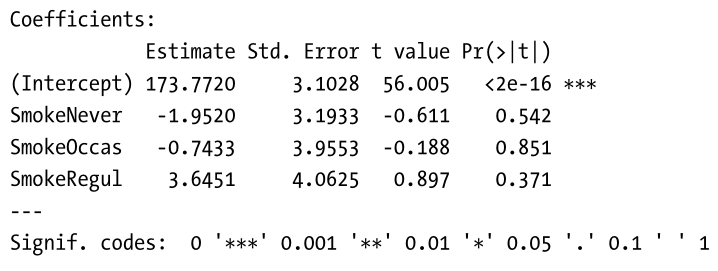
\includegraphics[scale =.7 ]  {figures/dummies_in_linear_model.png}}
\end{figure}



The observation in the reference category Heavy is represented solely
by $  \widehat{\beta}_{0} = 173.7720 $.




\section{Multiple Linear Regression}


\subsection{Terminology}

A {\underline {lurking variable}}, is what we've learned of the
{\underline {omitted variable}}. It can lead to a omitted variable bias.

A {\underline {nuisance or extraneous variable}} is a predictor of
no interest, but has the potential to confound (mess up) relationships
between other variables, and so affect your estimation. We are not
interested in it, but we {\underline {must}} add it to the model.


\subsection{The model}

\begin{equation*}
Y = \beta_0 + \beta_1 X_1 + \beta_2X_2 + ... + \beta_{p}X_{p} +
\varepsilon
\end{equation*}

You have $ n $ obs and $ p $ explanatory variables. For each obs, the
regression equation would be
\begin{equation*}
		y_{i} = \beta_0 + \beta_1x_{1,i} + \beta_2x_{2,i} + ... + 
		\beta_{p}x_{p,i} + \varepsilon_{i}
\end{equation*}
where $ i = 1,2,...,n $ stand for the $ i^{\text{ th }} $ obs.


{\textbf {Least-squared:}}
\begin{equation*}
\min_{\substack{\\}} \left( 
		\sum\limits_{i = 1} ^n(
		y_{i} - (\beta_0 + \beta_1x_{1,i} + \beta_2x_{2,i} + ... + 
		\beta_{p}x_{p,i})
		)	^{2}
\right)  
\end{equation*}


{\textbf {Matrix Form:}}
\begin{equation*}
\bm{Y} = \bm{X}\cdot \bm{\beta} + \bm{\varepsilon}
\end{equation*}
where $ \bm{Y} $ and $ \bm{\varepsilon} $ are $ n  \times 1 $ matrices
\begin{equation*}
\bm{Y} = 
\begin{bmatrix}
y_1\\y_2\\ \vdots  \\y_{n}
\end{bmatrix}
\quad
\text{ and }
\quad
\bm{\varepsilon} = 
\begin{bmatrix}
\varepsilon_1\\\varepsilon_2\\ \vdots  \\\varepsilon_{n}
\end{bmatrix}
\end{equation*}


\begin{equation*}
\bm{\beta} = 
\begin{bmatrix}
\beta_0\\\beta_1\\ \vdots \\\beta_{p}
\end{bmatrix}
\quad
\text{ and }
\quad
\bm{X} = 
\begin{bmatrix}
1 & x_{1,1} &\cdots&x_{p,1}\\
1 & x_{1,2} &\cdots&x_{p,2}\\
\vdots & \vdots &\ddots &\vdots \\
1 & x_{1,3} &\cdots&x_{p,3}\\
\end{bmatrix}
\end{equation*}


Matrix $ \bm{X} $ is $ n  \times (p + 1) $ dimension.


The OLS estimator $  \widehat{\bm{\beta}} $ :
\begin{equation*}
 \widehat{\bm{\beta}} = 
 \begin{bmatrix}
  \widehat{\beta}_{0}\\  \widehat{\beta}_{1}\\ \vdots \\  
	\widehat{\beta}_{p}
 \end{bmatrix}
 = (\bm{X}^{T}\cdot \bm{X})^{ - 1}\cdot \bm{X}^{T}\cdot \bm{Y}
\end{equation*}

\noindent\fbox{%
\parbox{\textwidth}{%
Derivation:
\begin{align*}
\min \bm{e}'\bm{e} &= \min \bm{(y - X   \widehat{\beta})'(y - X   \widehat{\beta})}\\
&= \bm{y'y - y'X  \widehat{\beta} -  \widehat{\beta}' X'y +  \widehat{\beta}'X'X 
 \widehat{\beta} }
\end{align*}
Note, $ \bm{ y'X  \widehat{\beta}} $, and $ \bm{ \widehat{\beta}' X'y} $ are scaler.
So the transpose of $ \bm{ y'X  \widehat{\beta}} $ is itself.
Remember the derivative of matrix: $ \frac{\partial \bm{x}'b }{\partial \bm{x} }
= b$

\begin{align*}
\frac{\partial \bm{e'e} }{\partial  \bm{\widehat{\beta}} }&= 0  
 - \frac{\partial (\bm{ \widehat{\beta}'X'y })' }{\partial \bm{ \widehat{\beta} } }
  - \bm{X'y} + 2 \bm{X'X  \widehat{\beta}} = 0\\
&= - \frac{\partial (\bm{ \widehat{\beta}'X'y }) }{\partial \bm{ \widehat{\beta} } }
  - \bm{X'y} + 2 \bm{X'X  \widehat{\beta}} = 0\\
&=  - \bm{X'y} - \bm{X'y} + 2\bm{X'X  \widehat{\beta}} = 0\\
2 \bm{X'X  \widehat{\beta}} &= 2 \bm{X'y}\\
\bm{ \widehat{\beta}}&= \bm{(X'X)^{ - 1}X'y}
\end{align*}
}%
}\\



\subsection{F-test}
For a regression below:
\begin{equation*}
y = \beta_0 + \beta_1x_1 + \beta_2x_2 + ... + \beta_{k}x_{k} + \varepsilon
\end{equation*}
we usually want to know the significance of the regression equation, i.e., whether
all $ \beta $s equal to zero.
So we need to do a  $ F $-test with null below:
\begin{equation*}
H_0: \beta_1 = ... = \beta_{k} = 0
\end{equation*}
This null hypothesis can be written in this way:
\begin{equation*}
H_0: \beta_1 = 0, \beta_2 = 0, ... \beta_{k} = 0
\end{equation*}

Write this into vector form:
\begin{equation*}
H_0:
\begin{pmatrix}
		1 & 0 & 0\\
		0 & 1 & 0\\
		0 & 0 & 1\\
\end{pmatrix}
\begin{pmatrix}
\beta_1\\
\beta_2\\
\beta_3\\
\end{pmatrix}
=
\begin{pmatrix}
0\\
0\\
0\\
\end{pmatrix}
\end{equation*}
Let 
\begin{equation*}
\bm{R}= 
\begin{pmatrix}
		1 & 0 & 0 & \cdots &0\\
		0 & 1 & 0 & \cdots &0\\
		0 & 0 & 1 & \cdots &0\\
		\cdots&\cdots&\cdots&\cdots &\cdots\\
		0 & 0 & 0 & \cdots &1\\
\end{pmatrix},
\bm{\beta}= 
\begin{pmatrix}
\beta_1\\
\beta_2\\
\beta_3\\
\cdots\\
\beta_{k}
\end{pmatrix}
\bm{r}= 
\begin{pmatrix}
0\\
0\\
0\\
\cdots\\
0
\end{pmatrix}
\end{equation*}

$ \bm{R}: K  \times K, \quad \bm{\beta}: K  \times 1, \quad \bm{r}: m  \times 1$ 
In this case m = K

So, the null can be written in this way,
\begin{equation*}
H_0: \bm{R} \bm{\beta} - \bm{r} = 0
\end{equation*}
We can use quadratic form representing the distance between it and 0 and do the Wald
test
\begin{equation*}
		\frac{(\bm{R} \bm{\beta - r}  - 0)^{2}}{Var(\bm{R \beta - r})} = 
		(\bm{R  \widehat{\beta} - r})'[Var(\bm{R  \widehat{\beta} - r})]^{ - 1}
		(\bm{R  \widehat{\beta} - r})'
\end{equation*}
Form the $ F $ statistics:
\begin{equation*}
F = \frac{
		[(\bm{R  \widehat{\beta} - r})'[Var(\bm{R  \widehat{\beta} - r})]^{ - 1}
		(\bm{R  \widehat{\beta} - r})']/m
}{s^{2}} \sim F(m,n - K)
\end{equation*}


Note, 
\begin{align*}
		Var(\bm{R  \widehat{\beta} - r})&= Var(\bm{R  \widehat{\beta}})\\
		&= \bm{R}Var( \widehat{\beta})\bm{R}'\\
		&= \sigma^{2}\bm{R}(\bm{X'X})^{ - 1}\bm{R}'
\end{align*}
We use $ s^{2} $ to estimate $ \sigma^{2} $.

If $ F $ is very large, p value would be small. If p value is smaller than $ \alpha $,
reject the null.

{\textbf {We can also use $ F $-test to test if two estimators are equal.}}\\

Example:

For model: $ y = \beta_1 + \beta_2x_2 + \beta_3x_3 + \beta_4x_4 + \varepsilon $,
if you want to test:
\begin{equation*}
H_0: \beta_2 = \beta_3, \beta_4 = 0
\end{equation*}
it can be written as
\begin{equation*}
H_0: \beta_2 - \beta_3 = 0, \quad \beta_4 = 0
\end{equation*}
\begin{equation*}
H_0:
\begin{pmatrix}
\beta_2 - \beta_3\\
\beta_4
\end{pmatrix}
=
\begin{pmatrix}
0\\
0
\end{pmatrix}
\end{equation*}
\begin{equation*}
H_0:
\begin{pmatrix}
0 & 1 &  -1 & 0\\
0 & 0 &  0 & 1
\end{pmatrix}
\begin{pmatrix}
\beta_1\\
\beta_2\\
\beta_3\\
\beta_4\\
\end{pmatrix}
=
\begin{pmatrix}
0\\
0
\end{pmatrix}
\end{equation*}
\begin{equation*}
\bm{R} = 
\begin{pmatrix}
0 & 1 &  -1 & 0\\
0 & 0 &  0 & 1
\end{pmatrix}
, \quad
\bm{\beta} = 
\begin{pmatrix}
\beta_1\\
\beta_2\\
\beta_3\\
\beta_4\\
\end{pmatrix}
, \quad
\bm{r} = 
\begin{pmatrix}
0\\
0
\end{pmatrix}
\end{equation*}













\subsection{Interpretation of the coef}

A coefficient for a specific variable should be interpreted as the
change in the mean response for a one-unit increase in the variable,
while {\underline {holding all other variables constant}}.




\subsection{Transformation}

Two ways to approach the transformation: 
{\underline {polynomial}} and {\underline {logarithmic}}.

The transformation in general does not represent a universal solution
to solving problems of {\underline {nonlinearity}} in the trend,
but it can at least {\underline {improve}} how faithfully a linear
model is able to represent those trends.



\subsubsection{Polynomial}
Add squared, cubic, and other polynomial terms to fit curved trend.
For example, 
\begin{equation*}
\text{ Income } = \beta_0 + \beta_1edu + \beta_2edu^{2} + 
\beta_3 exp + \beta_4exp^{2} + \varepsilon
\end{equation*}

Use $ I() $ function in R to add a polynomial term in $ lm() $ function.

{\textbf {Code:}}
\begin{rc}
lm_poly_result = lm(norm_price~norm_volume+norm_supply
+I(norm_supply**2),data = df)
summary(lm_poly_result)
\end{rc}


If the effect of adding one term is not good, we can try to add another 
cubic term and compare these two models.






\begin{table}[h!]
\begin{center}
	
\begin{threeparttable}
		\caption{Quadratic vs. Cubic term model}			

\begin{tabular}{lllll}
\\ [-1.8ex]
\hline
\hline \\[-1.8ex]
 & {\textbf {Model 1}} & {\textbf {Model 2}}  \\
\\ [-1.8ex]
\hline \\[-1.8ex]


(Intercept)      	&-0.024260   			&-0.095378 ***	 \\
									&(-1.523)    			&( -5.557)    	\\
norm\_volume      & 0.465420***			& 0.418280 ***	 \\ 
									&(28.338)    			&( 24.920)    	\\
norm\_supply      & 0.397987***			& 0.525587 ***	 \\ 
									&(24.030)    			&( 25.473)    	\\
I($norm\_supply^2$) & 0.024269*  			& 0.088337 ***	 \\ 
									&( 2.446)    			&(  7.588)    	\\
I($norm\_supply^3$) &                 &-0.030171 ***	\\
				          &                 &(-10.035)    	\\


\\ [-1.8ex]
\hline \\[-1.8ex]

\end{tabular}
\begin{tablenotes}
\small
\item Signif. codes:  0 ‘***’ 0.001 ‘**’ 0.01 ‘*’ 0.05 ‘.’ 0.1 ‘ ’ 1\\
\end{tablenotes}

\end{threeparttable}
\end{center}
\end{table}



Now we can see, by adding cubic term, the model performs better.


\subsubsection{Logarithmic}
Transforming to a logarithmic scale can help reduce the severity of
heavily {\underline {skewed}} data.




\subsection{Interaction Terms}

When estimating regression models, you always have to accompany 
interactions with the {\underline {main effect}} of the relevant
predictors.

In R, use a ``:"  specify an interaction term.

{\textbf {Code:}}

\begin{rc}
inter_lm_result = lm(
		norm_price~norm_volume+norm_supply+norm_volume:norm_supply,
		data = df
)
summary(inter_lm_result)
\end{rc}





\section{Linear Model Selection}

\subsection{Goodness of fit vs. Complexity}
{\textbf {GOF:}} refers to the goal of obtaining a model that best 
represents the relationships between the dependent and explanatory 
variables.\\

{\textbf {Complexity: }} how many terms (e.g., polynomial, etc) and
additional functions in your model. The more you have, the more 
complex the model would be.\\


{\textbf {The principle of parsimony:}} 
The balancing act between GOF and complexity.\\
Our goal is to find a model that is as simple as possible without
sacrificing too much GOF.\\
The model satisfies this notion is a {\underline {parsimonious fit}}.





\subsubsection{General Guideline}

1. You CANNOT remove individual levels of a categorical variable in 
a given model. Suppose college, master, phd are under edu, but only
phd are significant. You cannot remove the college and master. 
You can ONLY remove the entire categorical variable, i.e., edu.\\

2. If an interaction term is present in the fitted model, ALL lower-
order interactions and main effects of the relevant variables MUST
remain in the model. Suppose you add an interaction term,
$ edu  \times exp  \times age $, then the main effect ($ edu, exp,
age$) and all lower-order interaction terms ($ edu  \times exp,
edu  \times age, exp  \times age$) should be shown in the model.
Hence, in R, you'd better use $ VR_1*VR_2 $ for interaction term, so
that R will add all these terms for you. You will not miss any one of
them.\\

3. Keep ALL lower-order polynomial terms in the model if the highest
is deemed significant.



\subsection{Model Selection Algorithms}

\subsubsection{Nested Comparisons: The Partial F-Test}

It is the most direct way to compare several different models.
It looks at two or more {\underline {nested}} models.
The less complex model is a reduced version of the more complex model.
\begin{align*}
 \widehat{y}_{\text{ redu }} =  \widehat{\beta}_{0} +  
 \widehat{\beta}_{1}x_1  +  \widehat{\beta}_{2}x_2 + ... +
 \widehat{\beta}_{p}x_{p}\\
 \widehat{y}_{\text{ full }} =  \widehat{\beta}_{0} +  
 \widehat{\beta}_{1}x_1  + ... + ... \widehat{\beta}_{p}x_{p} + 
 ... +  \widehat{\beta}_{q}	x_{q}
\end{align*}

Clearly, $  \widehat{y}_{\text{ full }} $ is more complex than
$  \widehat{y}_{\text{ redu }} $, so we say that 
$  \widehat{y}_{\text{ redu }} $ is {\underline {nested}} within
$  \widehat{y}_{\text{ full }} $.

The {\textbf {partial F-Test}} tries to answer if it is worth it
to include any additional variables. Its goal is to test whether
include those extra $ q - p $ terms in $  \widehat{y}_{\text{ full }} $
provide a statistically significant improvement GOF.

\begin{align*}
H_0:& \beta_{p + 1} = \beta_{p + 2} = ... = \beta_{q} = 0\\
H_1:& \text{ At least one of the } \beta_{j} \ne 0 (\text{ for }
j = p,...,q)
\end{align*}


If the $ p $-value is less than the significant level, then we say
it is worth it because at least one of those extra $ q - p $ terms
is non-zero.


$ F $ statistics:
\begin{equation*}
F = \frac{
		(R_{\text{ full }}^{2} - R^{2}_{\text{ redu }}(n - q - 1))
}
{(1 - R^{2}_{\text{ full }})(q - p)}
\end{equation*}

It follows an $ F $ distribution with $ df_1 = q - p $, 
$ df_2 = n - q $ degree of freedom. The $ p $-value is found as the
{\underline {upper-tail}} area from $ F $ as usual.\\


In R, we can use $ anova(\text{ model1, model2 }) $ to conduct a
partial $ F $ -test.
We pass the {\underline {reduced}} model first, then the complex model.

{\textbf {Code:}}
\begin{rc}
redu_model = lm(norm_price~norm_volume+norm_supply, data = df)
complex_model = lm(norm_price~norm_volume*norm_supply, data = df)
anova(redu_model, complex_model)
\end{rc}

In the complex model, instead of the main effect, we add interaction 
term of these two. And the result shows that this additional interaction
term do provide a statistically significant improvement in fit because
the $ p $-value is pretty small. We reject the null.

The number of variables in the reduced model is $ p = 2 $, and the
number of variables in the complex model is $ q = 3 $ (two main effects
and a interaction term). Hence we can compute the DF (degree of 
freedom), $ DF = q - p = 3 - 2 = 1 $. And that is shown in the second
row of the table, i.e., column DF.

From the result, statistics $ F = 15.717 $, $ df_{1} = 1 $, 
$ df_2 = 2569 $.

{\textbf {Again,}} we use the partial $ F $-test to verify if the
complex model provides an improvement in fit.


{\textbf {Disadvantage:}} It can be difficult to manage if you have
many different models to fit when you have many explanatory variables.
{\underline {Forward Selection}} can help us to deal with this problem.






\begin{table}[h!]
\begin{center}
	
\begin{threeparttable}
		\caption{The Partial F-test result}			

\begin{tabular}{llllll}
\\ [-1.8ex]
\hline
\hline


\hline \\[-1.8ex]
 & {\textbf {Res.DF}} & {\textbf {RSS}} &{\textbf {DF}}&{\textbf {F}} & 
 {\textbf {p-value}}  \\
\\ [-1.8ex]
\hline \\[-1.8ex]


Model 1   &2570 &1029.8			&   &				&\\
Model 2   &2569 &1023.6     &1  &15.717 &7.556e-05 ***\\




\\ [-1.8ex]
\hline \\[-1.8ex]

\end{tabular}
\begin{tablenotes}
\small
\item Signif. codes:  0 ‘***’ 0.001 ‘**’ 0.01 ‘*’ 0.05 ‘.’ 0.1 ‘ ’ 1
\item Model 1: norm\_price = norm\_volume + norm\_supply
\item Model 2: norm\_price = norm\_volume * norm\_supply
\end{tablenotes}

\end{threeparttable}
\end{center}
\end{table}






\subsubsection{Forward Selection}


Also called forward elimination.

{\textbf {Step 1:}}\\
It starts with an {\underline {intercept-only}} model, and then
perform a series of independent tests to determine which of your 
explanatory variables significantly improves the GOF.

{\textbf {Step 2:}}\\
Then you add that term and execute the series of tests again for
all remaining terms to determine which of those would further improve
the fit.

{\textbf {Step 3:}}\\
The loop stops until there's no term can further improve the GOF.\\



Table below shows the result of intercept-only model. 


\begin{table}[h!]
\begin{center}
	
\begin{threeparttable}
		\caption{Intercept-only model}			
\begin{tabular}{ccccc}
\\ [-1.8ex]
\hline
\hline

\hline \\[-1.8ex]
 & {\textbf {Coef}} & {\textbf {Se}} &{\textbf {t-value}}&{\textbf {p-value}} \\
\\ [-1.8ex]
\hline \\[-1.8ex]


Intercept &-2.036e-16  &1.971e-02       &0        &1\\



\\ [-1.8ex]
\hline \\[-1.8ex]

\end{tabular}
\begin{tablenotes}
\small
\item Signif. codes:  0 ‘***’ 0.001 ‘**’ 0.01 ‘*’ 0.05 ‘.’ 0.1 ‘ ’ 1
\end{tablenotes}

\end{threeparttable}
\end{center}
\end{table}




Now we use $ add1() $ to find the most helpful variable to be added to
our intercept-only model.





\begin{table}[h!]
\begin{center}
	
\begin{threeparttable}
		\caption{Forward selection}			
\begin{tabular}{ccccccc}
\\ [-1.8ex]
\hline
\hline

\hline \\[-1.8ex]
 & {\textbf {DF}} & {\textbf {Sum of Sq}} &{\textbf {RSS}}&
{\textbf {ACI}} & {\textbf {F-value}} & {\textbf {p-value}} \\
\\ [-1.8ex]
\hline \\[-1.8ex]

none       &     &       &2572.0 & 1.0     &       & \\
norm\_supply  &1    &1173.3 &1398.7 &-1564.4  &2156.8 &$<$ 2.2e-16 ***\\
norm\_volume  &1    &1301.8 &1270.2 &-1812.3  &2635.0 &$<$ 2.2e-16 ***\\


\\ [-1.8ex]
\hline \\[-1.8ex]

\end{tabular}
\begin{tablenotes}
\small
\item Signif. codes:  0 ‘***’ 0.001 ‘**’ 0.01 ‘*’ 0.05 ‘.’ 0.1 ‘ ’ 1
\end{tablenotes}

\end{threeparttable}
\end{center}
\end{table}


From we want to add the one with ``three stars". Let's add norm\_
supply first. Then you keep doing this. The R code is below.


{\textbf {Code:}}
\begin{rc}
model1 = lm(norm\_price~1, data = df)
summary(model1)

add1(model1, scope = .~.+norm\_supply+norm\_volume, test = 'F')

model2 = update(model1, formula = .~. + norm\_supply)
summary(model2)

add1(model2, scope = .~.+norm\_volume, test = 'F')
\end{rc}










\subsubsection{Backward Selection}

As a reverse of the {\underline {Forward Selection}}, Backward Selection
starts with your full/complex model, and systematically drops terms.

In R, we instead of $ add1() $, we use $ drop1() $for backward 
selection and conduct the partial $ F $-test and $ update() $.
In contrast with the adding terms in forward selection, here we are
going to drop those terms DO NOT result in a {\underline {statistically
significant}} detriment to GOF.  We drop those terms do not have
``stars" in the result of $ drop1() $.


{\textbf {Code:}}
\begin{rc}
model1 = lm(norm_price~norm_volume*norm_supply, data = df)
summary(model1)
drop1(model1, test = 'F')
# use update(model1, .~.-norm_volume*norm_supply) to drop a term.
# Since this interaction term is significant, we don't want to drop it.
\end{rc}



\subsubsection{Stepwise AIC Selection}


The partial $ F $-test is the most common {\underline {test-based}}
model selection method.\\
Besides it, we also have a {\underline {criterion-based}} approach.
One of them is known as Akaike's Information Criterion, or 
{\underline {AIC}} for short.

For a given lnear model, AIC is calculated as follows:
\begin{equation*}
AIC =  - 2  \times \mathscr{L} + 2  \times (p + 2),
\end{equation*}
where $ \mathscr{L} $ is a measure of GOF named the 
{\underline {log-likelihood}}, and $ p $ is the number of regression
parameters in the model, excluding the overall intercept
(explanatory variables).
A smaller values of AIC refer to more parsimonious models.

{\textbf {NOTE:}} The value of AIC has no direct interpretation and
is useful ONLY when you compare it against the AIC of another model.
Hence, you can decide on which term to add or drop based on the change
of the AIC values, instead of focusing exclusively on the significance
of the change via the $ F $-test when you conduct a 
{\underline {forward or backward selection}}.\\

You can implement stepwise AIC selection yourself by using either
add1 or drop1 at each stage, but forfunately R provides the built-in
step function for you.

{\textbf {Progress:}}\\
You can start with any model you like. Here, let's start with the
intercept-only model.\\

{\textbf {Code:}}
\begin{rc}
model1 = lm(norm_price~1, data = df)
stepwise_model_selection = step(model1, 
				scope = .~. + norm_volume*norm_supply
)
summary(stepwise_model_selection)
\end{rc}


R would return a list of results, each block of them starts with a 
regression model and its AIC value, and presents the change of AIC
by adding or deleting a term $ ( + , - ) $. 

The {\underline {final model}} is stored, and you can check it using
$ sumamry() $. 

{\textbf {Note:}}\\
The AIC is sometimes criticized for a tendency to err on the side of
more complexity and higher $ p $-values. To balance this, you can 
{\underline {increase}} the penalizing effect by increasing the
multiplicative contribution of $ p + 2 $ on the RHS. Now is 
$ 2  \times (p + 2) $, you can try $ 2.5  \times (p + 2) $, etc.

Criterion-based measures are incredibly useful when you have models that
aren't nested (ruling out the partial $ F $-test).




\subsubsection{BIC selction algorithm}
Besides AIC, the corrected AIC ($ AIC_{c}) $ and the BIC
(Bayesian Information Criterion) are alternatives to AIC. They
impose heavier penalties on complexity than the default AIC.

Also, the adjusted $ R^{2} $ is another selection algorithm. Recall,
$ R^{2} $ does not penalize the complexity, but, here, the adjusted
$ R^{2} $ does incorporate a penalty for complexity relative to 
the sample size $ n $.
\begin{equation*}
		\overline{R}^{2} = 1  - \frac{(1 - R^{2})(n - 1)}
		{n - p - 1},
\end{equation*}
where $ p $ is the number of predictor terms. Monitoring
$  \overline{R}^{2} $ can be useful as a quick check between nested 
models -- {\underline {a higher value}} points to a preferred model.




\subsection{Residual Diagnostics}

We are going to cover the methods that are essential for determining
the {\underline {validity}} of your model, 
{\underline {model diagnostics}}.
The {\underline {goal}} is to ensure that your model is 
{\underline {valid and accurately}} represents the relationships in
your data.



\subsubsection{Inspecting and Interpreting Residuals}

We can plot a scatterplot of the {\underline {observed-minus-fitted}}
raw residuals. By assumption, they should appear randomly around zero.
This plot can also be used to detect {\underline {heteroscedasticity}}.

\begin{figure}[H]
\center{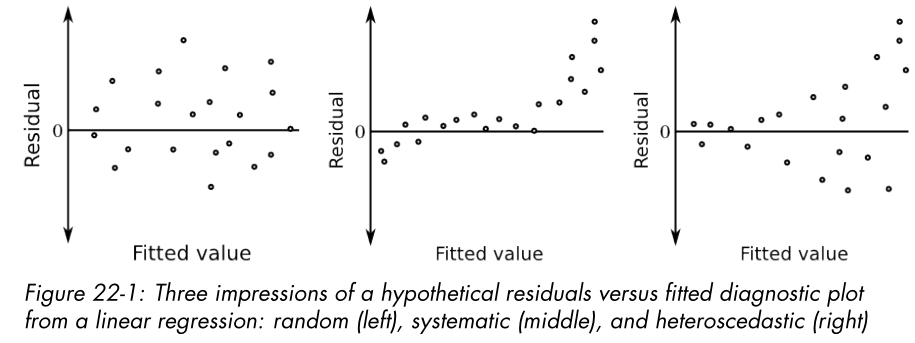
\includegraphics[scale =.6 ]  {figures/scatterplot_residuals.png}}
\end{figure}

The figure above shows the scatterplot of the residuals. The one on 
the left shows a homoscedasticity, good. The one on the right
is a heteroscedasticity result.


{\textbf {Note:}}\\
Even if your result does not like the figure on the left, you can still
improve your model by adding explanatory variable, changing the
treatment of a categorical variable, or performing nonlinear
transformations of certain continuous variables to reduce 
nonlinearity.

In R, you can use {\underline {plot()}} function on a 
{\underline {lm()}} object, it can produce six types of diagnostic
plot of the fit. You can {\underline {manually select}} a particular
plot specifying {\underline {which = i}} argument, where $ i $ stands
for the $ i^{\text{ th }} $ plot.


{\textbf {Code:}}
\begin{rc}
model1 = lm(norm_price~norm_supply*norm_volume, data = df)
png('figures/residual_diagnostic_plots.png')
par(mfrow = c(2,3))
plot(model1, which = 1)
plot(model1, which = 2)
plot(model1, which = 3)
plot(model1, which = 4)
plot(model1, which = 5)
plot(model1, which = 6)
dev.off()
\end{rc}


\begin{figure}[H]
\caption{Six types of diagnostic plots.}
\center{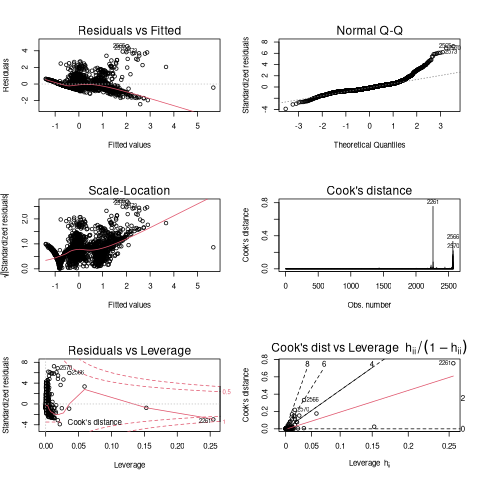
\includegraphics[scale =.8 ]  {figures/residual_diagnostic_plots.png}}
\end{figure}

The scale-location plot provides
\begin{equation*}
\left\lvert 
		\frac{e_{i}}{ \widehat{\sigma}\left\{ 1 - h_{ii} \right\}
		^{\frac{1}{2}} }
\right\rvert ^{\frac{1}{2}}
\end{equation*}

It is used to reveal tends in the size of the {\underline {
departure}} of each data point from its fitted value. It is much more
useful than the raw residuals in detecting things such as
{\underline {heteroscedasticity}}.




\subsubsection{Assessing Normality}

You can use a normal QQ plot (pass $ which = 2 $) to check the 
normality.

\begin{rc}
model1 = lm(norm_price~norm_supply*norm_volume, data = df)
plot(model1, which = 2)
\end{rc}




There are also other ways to test for normality, such as Shapiro-Wilk
test.
The null is that the data are normally distributed. We can use
$ shapiro.test() $ in R to implement this test.


{\textbf {Code:}}
\begin{rc}
model1 = lm(norm_price~norm_volume*norm_supply, df)
shapiro.test(rstandard(model1))
#         Shapiro-Wilk normality test
# 
# data:  rstandard(model1)
# W = 0.84736, p-value < 2.2e-16
# Here, we reject the null, hence, the data are not normally distributed. 
\end{rc}




\subsubsection{Illustrating outliers, leverage, and influence}

{\textbf {Leverage:}}\\
The extremity of the values of the {\underline {explanatory variable}}.
A high-leverage point is an {\underline {observation}} with 
explanatory values extreme enough to potentially 
{\underline {significantly affect}} the slopes or trends in the fitted
model.\\
An outlier can have a high or low leverage.\\

{\textbf {Influence:}}\\
An obs with high leverage that DOES affect the estimated trends is
deemed influential.\\

{\textbf {Example:}}\\
The figure below shows how outlier with different leverage level affect
the regression model.


\begin{figure}[H]
		\center{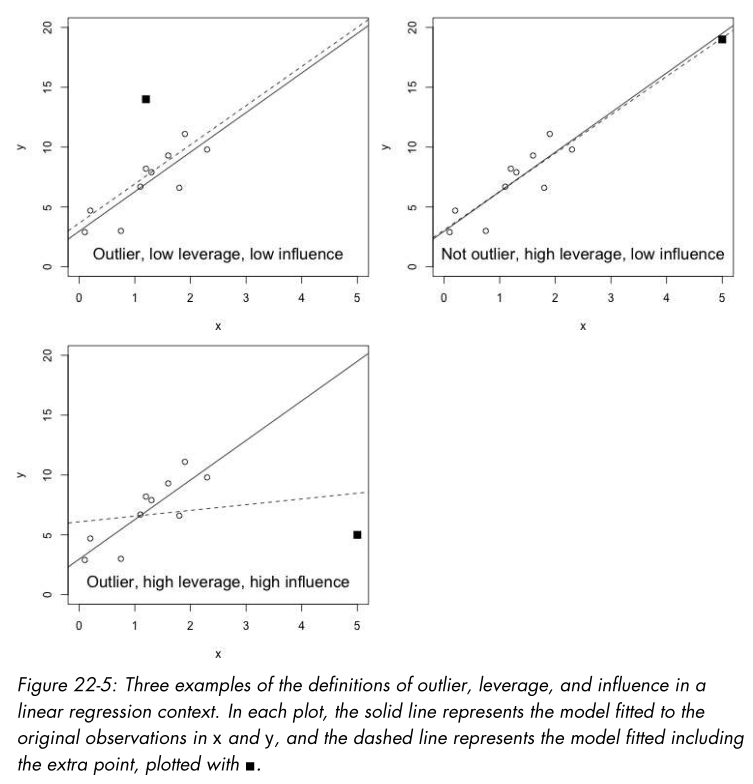
\includegraphics[scale =0.7 ]  {figures/outlier_leverage_influence.png}}
\end{figure}



The solid black brick stands for different outliers. The solid line
represent the original regression line while the dash line present
the new regression line as a result of including the outlier.




\subsubsection{Calculating Leverage}


With $ n $ obs, the leverage of the $ i $th point ($ i = 1,...,n $ )
is denoted $ h_{ii} $. These are {\underline {diagonal}} elements
of the $ n  \times n $ matrix $ H $ ($ i $th row and $ i $th column).
\begin{equation*}
H = \bm{X}(\bm{X}^{T}\bm{X})^{ - 1}\bm{X}^{T}
\end{equation*}


In R, you can use $ hatvalues() $ and pass your regression model to
obtain the leverage.

{\textbf {Code:}}\\
\begin{rc}
model0 = lm(norm_price~norm_volume, data = df)
vol_leverage = hatvalues(model0)
\end{rc}



\begin{figure}[H]
		\center{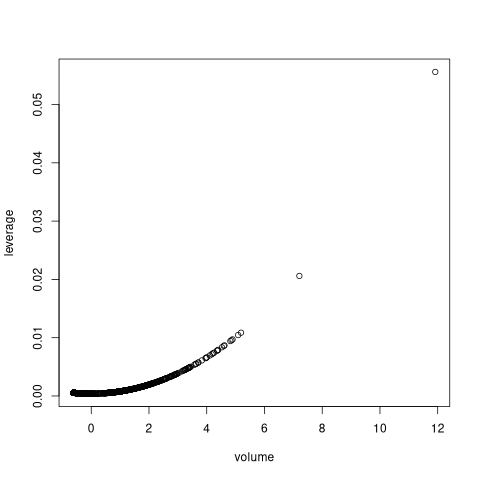
\includegraphics[scale =.5 ]  {figures/volume_leverage.png}}
\end{figure}




\subsubsection{Cook's Distance}

Leverage is not enough to determine the overall {\underline {influence}} 
of each obs on a fitted model. We can use {\underline {Cook's
Distance}} to measure the influence.

\begin{equation*}
D_{i} = \sum\limits_{j = 1} ^n
\frac{( \widehat{y}_{j} -  \widehat{y}_{j}^{ (- i)})^{2}}
{(p + 1) \widehat{\sigma}^{2}}, 
\quad i,j = 1,...,n,
\end{equation*}


where $  \widehat{y}_{j}^{( - i)} $ represents the estimated value
of obs $ j $ {\underline {without}} the $ i $th observation. And
$ p $ is the number of explanatory variables, 
$   \widehat{\sigma}^{2} $ is the estimated variance.

The larger the value of $ D_{i} $, the larger the influence the 
$ i $th observation has on the fitted model. 
Some people say if $ D_{i} > 1 $, the point should be considered
influential. Another argument is that $ D_{i} > \frac{4}{n} $.

In R, use cooks.distance() to implement the cook's distance.


{\textbf {Code:}}\\
\begin{rc}
cook = cooks.distance(model0)
png('figures/cooks_distance_vol.png')
plot(norm_volume, cook, data = df, xlab = 'volume', ylab = 'cooks')
dev.off()
\end{rc}


\begin{figure}[H]
		\center{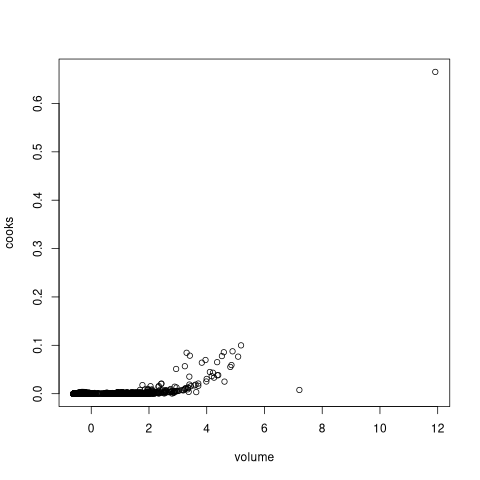
\includegraphics[scale =.4 ]  {figures/cooks_distance_vol.png}}
\end{figure}


Or you can use plot(regression model, which = 4) to plot cooks 
distance.

\begin{figure}[H]
		\center{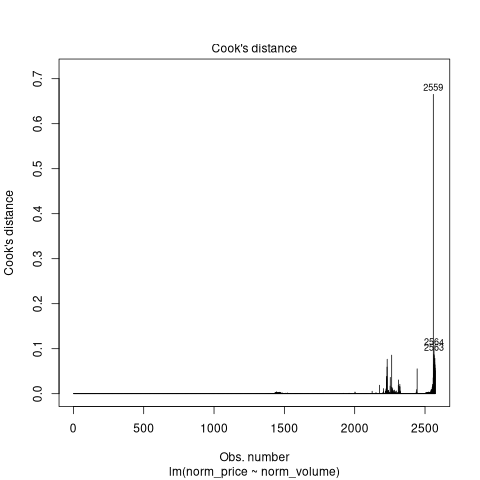
\includegraphics[scale =0.4 ]  {figures/cooks_distance_built_in_plot.png}}
\end{figure}


We can further implement that $ D_{i} > \frac{4}{n} $ rule in the plot.

\begin{figure}[H]
		\center{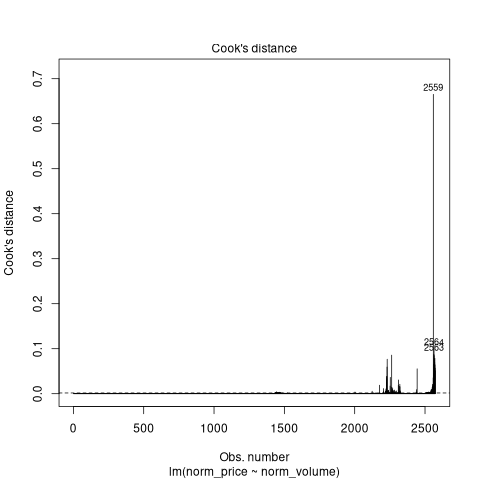
\includegraphics[scale =.5 ]  {figures/cooks_distance_with_4-n.png}}
\end{figure}





\subsection{Collinearity}

Collinearity, also called multicollinearity, happends when two or
more of the explanatory variables are highly correlated with each 
other. It would be detrimental to any subsequent model-based 
inference.

\subsubsection{Signal of the collinearity}
1. $ F $-test result is significant, but none of the individual
$ t $-test results are significant.\\

2. The sign of a given coef estimate contradicts what you would 
reasonably expect to see, e.g., drinking more wine resulting in a 
lower blood alcohol level.\\

3. Estimators are associated with unusually high SE or vary wildly when
the model is fitted to differnt random record subsets of the data.\\



{\textbf {Note:}}\\

If two or more {\underline {explanatory variables}} in your model
are collinear, then the estimates (coef) of regress $ y $ on each of
them respectively would be almost the same.































\end{document}

